\section{Durchführung}
\label{sec:Durchführung}
Zur Messung einer Kennlinienschar der Hochvakuumdiode wird für fünf
verschiedene Heizleistungen zwischen $\SI{2}{\ampere}$ und $\SI{2.5}{\ampere}$
jeweils eine Kennlinie aufgenommen. Die Messung wird mittels eines Amperemeters
und Voltmeters durchgeführt. Die hierfür verwendete Schaltung ist folgender
Abbildung zu entnehmen.
\begin{figure}[H]
  \centering
  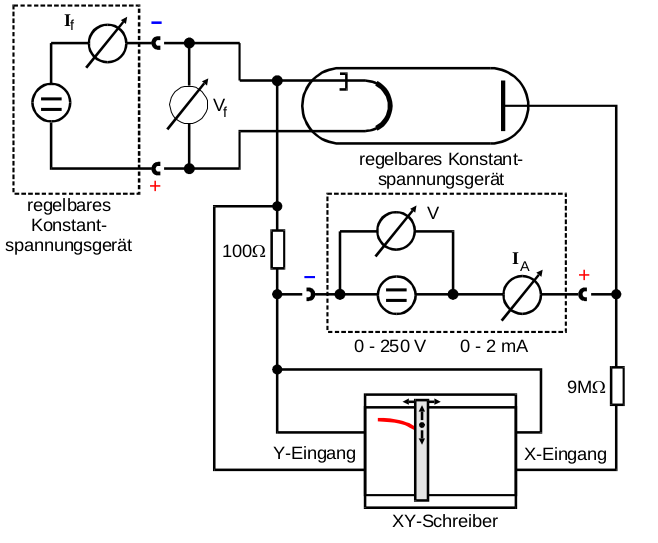
\includegraphics[scale=0.5]{content/schaltungkennlinie.png}
  \label{fig:schaltungkennlinie}
  \caption{Die zur Kennlinienaufnahme verwendete Schaltung. \cite{AP01}}
\end{figure}
\noindent
Zur Untersuchung des Anlaufstromgebietes wird folgende Schaltung verwendet:
\begin{figure}[H]
  \centering
  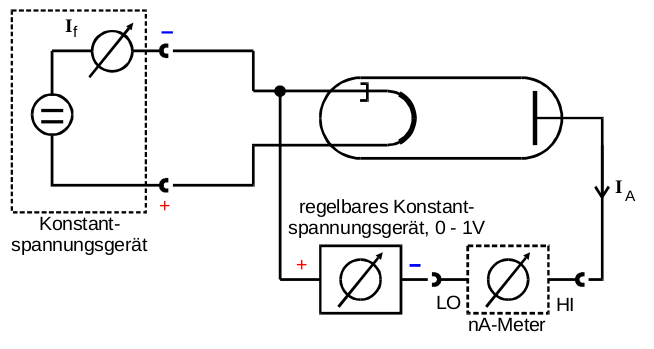
\includegraphics[scale=0.5]{content/schaltunganlaufstromgebiet.png}
  \label{fig:schaltunganlaufstrom}
  \caption{Die verwendete Schaltung für die Untersuchung des Anlaufstromgebietes.\cite{AP01}}
\end{figure}
\noindent
Hierbei wird in $\SI{0.1}{\ampere}$-Schritten von $\SI{0}{\ampere}$ bis
$\SI{1}{\ampere}$ Diodenstrom die Anodenstromstärke gemessen.
